\documentclass[tikz,border=5pt]{standalone}
\usepackage{tikz}
\usepackage{cancel}
\usepackage{amsfonts}
\usetikzlibrary{arrows.meta}

\begin{document}

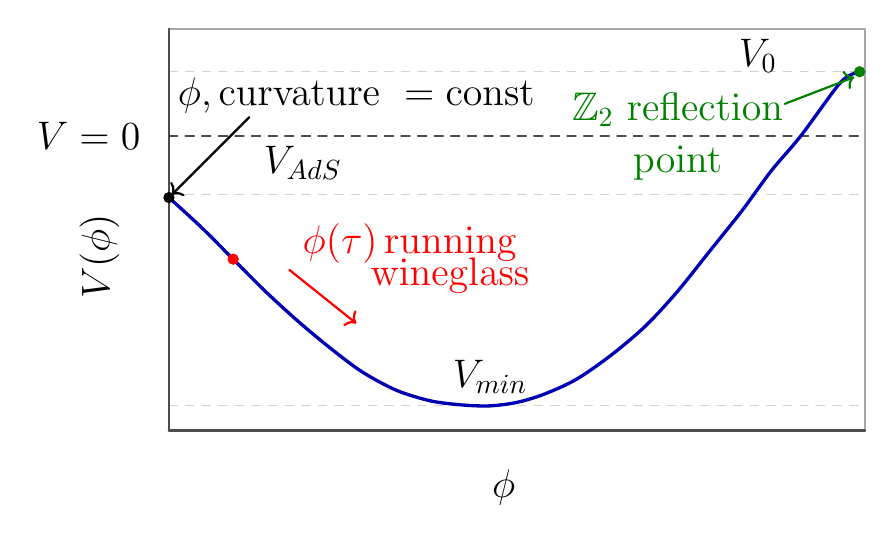
\begin{tikzpicture}[scale=0.34, line cap=round, line join=round]

% Frame
\draw[gray!70, line width=0.8pt] (0,0) rectangle (26,15);

% Background gridlines
\draw[gray!35, dashed] (0,13.4) -- (26,13.4);
\draw[gray!35, dashed] (0,8.8) -- (26,8.8);
\draw[gray!35, dashed] (0,0.92) -- (26,0.92);
\draw[black!65, line width=0.7pt, dashed] (0,11) -- (26,11);

% Axes
\draw[black!70, line width=0.9pt] (0,0) -- (26,0);
\draw[black!70, line width=0.9pt] (0,0) -- (0,15);
\draw[black!70, line width=0.7pt, dashed] (0,11) -- (26,11);


% Single smooth curve
\draw[blue!70!black, line width=1.2pt, smooth]
  plot coordinates {
    (0.0,8.7)
    (1.2,7.6)
    (2.4,6.4)
    (3.6,5.2)
    (4.8,4.1)
    (6.0,3.1)
    (7.2,2.2)
    (8.5,1.5)
    (9.8,1.1)
    (11.0,0.95)
    (12.0,0.92)
    (13.0,1.05)
    (14.0,1.35)
    (15.2,1.9)
    (16.5,2.8)
    (17.8,3.9)
    (19.0,5.2)
    (20.2,6.7)
    (21.4,8.2)
    (22.5,9.7)
    (23.6,11.0)
    (25,12.9)
    (25.5,13.3)
    (25.8,13.4)
  };

% Axis labels
\node[below, font=\Large] at (12.5,-1.1) {$\phi$};
\node[rotate=90, font=\Large] at (-2.6,6.5) {$V(\phi)$};

% Text inside the plot
\node[font=\Large] at (-3,11) {$V=0$};
\node[font=\Large] at (22,14) {$V_0$};
\node[font=\Large] at (5,10) {$V_{AdS}$};
\node[font=\Large] at (12,2) {$V_{min}$};
\fill[red] (2.4,6.4) circle (6pt);
\node[font=\Large] at (9,7) {$\color{red}\phi(\tau)\,\rm running$};
\node[font=\Large] at (10.5,5.8) {$\color{red}\rm wineglass$};
\draw[->, red, thick] (4.5,6) -- (7,4);
\fill[green!50!black] (25.8,13.4) circle (6pt);
\draw[->, green!50!black, thick] (23,12.2) -- (25.6,13.2);
\node[font=\Large] at (19,12) {$\color{green!50!black} \mathbb{Z}_2~\rm {reflection}$};
\node[font=\Large] at (19,10) {$\color{green!50!black} \rm {point}$};
\fill[black] (0.0,8.7) circle (6pt);
\draw[->, black, thick] (3,11.7) -- (0.1,8.8);
\node[font=\Large] at (7,12.5) {$\color{black} \phi, \rm{curvature}~\rm = const $};
\end{tikzpicture}

\end{document}